\chapter{Contexte Général et Cadre Méthodologique}
\section*{Introduction}
\phantomsection
\addcontentsline{toc}{section}{Introduction}

Ce premier chapitre pose le cadre du projet Smart Farm AI : présentation
de l'entreprise d'accueil, analyse du contexte agricole tunisien, étude
de l'existant, définition des objectifs et description de la méthodologie
adoptée.

% ── 1.1 Organisme d'accueil ─────────────────────────────────
\section{Organisme d'accueil : Intech Solutions}

\subsection{Présentation générale}
\textbf{Intech Solutions} est une entreprise tunisienne de services numériques
spécialisée dans le développement de solutions intelligentes pour les secteurs
agro-industriels et agroalimentaires. Fondée à Sfax, elle s'est positionnée
sur le créneau porteur de l'agri-tech nationale en proposant des solutions
IoT, des plateformes SaaS et des services d'intégration IA adaptés aux
contraintes des exploitations tunisiennes.

\begin{figure}[H]
\centering

\includegraphics[width=0.45\textwidth]{figures/logo_intech_solutions.png}
\caption[Logo InTech Solutions]{Logo de l'entreprise d'accueil Intech Solutions}
\label{fig:logo_intech_solutions}
\end{figure}


\subsection{Domaines d'expertise}

InTech Solutions intervient comme intégrateur IT régional en Tunisie et en
Égypte, avec une offre structurée autour de l'infrastructure, de la sécurité,
des solutions ERP, de l'infonuagique, des centres de données et de l'intelligence artificielle.
Depuis sa création en 2018, l'entreprise accompagne les organisations dans la
conception, le déploiement et l'exploitation d'environnements technologiques
sur mesure, en intégrant l'IA dans ses processus de livraison, ses opérations et
les plateformes développées pour ses clients.

Le tableau~\ref{tab:domaines_expertise_intech} synthétise les principaux domaines d'expertise de l'entreprise.

\begin{table}[H]
\centering
\caption{Domaines d'expertise d'InTech Solutions}
\label{tab:domaines_expertise_intech}
\renewcommand{\arraystretch}{1.25}
\resizebox{\textwidth}{!}{%
\begin{tabular}{p{0.30\textwidth}p{0.64\textwidth}}
\toprule
\textbf{Domaine d'expertise} & \textbf{Périmètre d'intervention} \\
\midrule
Intelligence artificielle et automatisation &
Copilotes et assistants IA, automatisation documentaire, prévision, analyse de données, détection d'anomalies et recherche intelligente de type RAG. \\
\addlinespace
Intégration de solutions informatiques &
Architecture système, intégration de systèmes hétérogènes, migration de données et interconnexion de plateformes métiers. \\
\addlinespace
Solutions de centres de données et infrastructure &
Armoires intelligentes, serveurs, stockage, virtualisation, conteneurs, postes virtuels et supervision d'environnements critiques. \\
\addlinespace
Solutions ERP et plateformes métier &
Intégration Odoo, gestion commerciale, finance, ressources humaines, production, chaîne logistique et plateformes SaaS augmentées par l'IA. \\
\addlinespace
Informatique en nuage et cybersécurité &
Migration vers le nuage, sauvegarde, architectures hybrides, configuration de pare-feu, sécurité des terminaux, tests d'intrusion et défense en profondeur. \\
\addlinespace
Développement logiciel et web &
Sites, portails, applications métier et interfaces web modernes intégrant des fonctionnalités IA dès la phase de conception. \\
\addlinespace
Maintenance, assistance et conseil &
Maintenance proactive, assistance à distance, surveillance de l'état des systèmes, audit informatique, schémas directeurs et transformation numérique. \\
\addlinespace
Systèmes de sécurité et sûreté &
Vidéosurveillance, contrôle d'accès, détection d'intrusion, détection incendie et intégration de solutions de sûreté physique. \\
\bottomrule
\end{tabular}%
}
\end{table}

Cette couverture fonctionnelle est renforcée par un écosystème de plateformes
et de produits associés, notamment TaskFuze, EasyFacture, EasySign,
InTelligencia BI, InTunnel et RFID Inventory, ainsi que par un réseau de
partenaires technologiques incluant des acteurs majeurs tels que Lenovo, Dell
EMC, HPE, Cisco, Fortinet, Microsoft, AWS, Odoo, DigitalOcean et Google
Workspace.

\subsection{Informations clés sur InTech Solutions Tunisie}

Le tableau~\ref{tab:infos_cles_intech} présente une synthèse des informations
institutionnelles disponibles sur InTech Solutions Tunisie.

\begin{table}[H]
\centering
\caption[Informations clés InTech]{Informations clés sur InTech Solutions Tunisie}
\label{tab:infos_cles_intech}
\renewcommand{\arraystretch}{1.25}
\begin{tabular}{p{0.32\textwidth}p{0.58\textwidth}}
\toprule
\textbf{Élément} & \textbf{Détails} \\
\midrule
Adresse & N\textsuperscript{o} 14 Marsa Mall, La Marsa, Tunis 2046, Tunisie. \\
Courriel & contact@intech-eg.tech \\
Téléphone & +216 70 137 920 / +216 56 373 373 \\
Site Internet & Site institutionnel InTech Solutions TN. \\
Année d'implantation & 2018. \\
Nombre d'employés & 15 collaborateurs, répartis entre direction, développement logiciel, opérations techniques, finance et développement commercial. \\
Parts de marché & Donnée non publiée ; l'entreprise revendique toutefois plus de 250 projets livrés, plus de 20 secteurs servis et un réseau de 38 partenaires technologiques. \\
\bottomrule
\end{tabular}
\end{table}

\subsection{Structure organisationnelle}

L'organisation interne d'InTech Solutions repose sur une équipe pluridisciplinaire
associant direction, ingénierie logicielle, opérations techniques, finance et
développement commercial. Le tableau~\ref{tab:structure_org_intech} synthétise
les principales fonctions identifiées.

\begin{table}[H]
\centering
\caption{Structure organisationnelle d'InTech Solutions Tunisie}
\label{tab:structure_org_intech}
\renewcommand{\arraystretch}{1.25}
\resizebox{\textwidth}{!}{%
\begin{tabular}{p{0.24\textwidth}p{0.30\textwidth}p{0.38\textwidth}}
\toprule
\textbf{Pôle} & \textbf{Responsables / profils} & \textbf{Rôle principal} \\
\midrule
Direction générale & Abdelrahman Nasser, Cyrine Ben Haj Ali, Amine Ben Sassi & Pilotage stratégique, gestion opérationnelle, architecture projet, gouvernance financière et développement de l'entreprise. \\
\addlinespace
Développement commercial & Zied Haddad & Prospection, développement des partenariats, négociation commerciale et analyse des opportunités de marché. \\
\addlinespace
Ingénierie logicielle & Manel Ben Sassi, Ines Soltani, Jihen Hasnaoui, Med Amine Chérif, Wadii Dridi & Développement web et logiciel, intégration ERP, interfaces frontales, API, bases de données, applications métier et fonctionnalités IA. \\
\addlinespace
Finance et administration & Sarra Ben Haj Ali & Planification financière, suivi budgétaire, gestion des risques et appui à la croissance de l'entreprise. \\
\addlinespace
Opérations techniques & Sami Boukhili, Marouen Harrouchi, Amine Helali, Walid Majdoub, Youssef Chehid & Assistance informatique, infrastructure réseau, systèmes, cybersécurité, vidéosurveillance, maintenance et assistance technique aux clients. \\
\bottomrule
\end{tabular}%
}
\end{table}

\subsection{Vision stratégique}
La vision d'Intech Solutions s'articule autour du concept de
\textbf{souveraineté numérique agricole} : offrir aux agriculteurs tunisiens
des outils performants, économiques (open-source), en leur langue maternelle,
sans dépendance vis-à-vis des API propriétaires étrangères. Cette vision
a directement guidé les choix architecturaux du projet (Ollama local,
modèles embarqués, RBAC strict).

% ── 1.2 Contexte du projet ──────────────────────────────────
\section{Contexte du projet}

\subsection{Étude de l'existant}

Le secteur de l'agriculture intelligente connaît une évolution rapide sous
l'effet de l'IoT, de l'intelligence artificielle, des plateformes ERP et des
applications mobiles. Plusieurs solutions internationales proposent déjà des
fonctionnalités de gestion agricole, de suivi de production, d'aide à la
décision ou de supervision terrain. Toutefois, ces solutions restent souvent
centrées sur des marchés à forte maturité numérique et ne répondent pas
pleinement aux contraintes des exploitations tunisiennes, notamment en matière
de coût, de langue, de connectivité et de souveraineté des données.

\begin{table}[H]
\centering
\caption{Comparaison des solutions d'agriculture intelligente existantes}
\label{tab:comparaison_existant}
\resizebox{\textwidth}{!}{%
\begin{tabular}{lccccc}
\toprule
\textbf{Critère} & \textbf{Smart Farm AI} & \textbf{Trimble Ag} & \textbf{FieldView} &
  \textbf{FarmERP} & \textbf{AgriWebb} \\
\midrule
IoT intégré      & \checkmark & \checkmark & \checkmark & \texttimes & \checkmark \\
IA locale        & \checkmark & \texttimes & \texttimes & \texttimes & \texttimes \\
Prise en charge de la Darija & \checkmark & \texttimes & \texttimes & \texttimes & \texttimes \\
Code source ouvert & \checkmark & \texttimes & \texttimes & Partiel    & \texttimes \\
Module apiculture& \checkmark & \texttimes & \texttimes & \texttimes & \texttimes \\
ERP avicole      & \checkmark & \texttimes & \checkmark & \checkmark & \texttimes \\
PWA hors connexion & \checkmark & \texttimes & \texttimes & \texttimes & \texttimes \\
Coût annuel (USD)& \$0        & \$3\,000+  & \$1\,500+  & \$2\,000+  & \$1\,200+ \\
\bottomrule
\end{tabular}%
}
\end{table}

\subsection{Problématique}

L'analyse de l'existant révèle que les solutions disponibles présentent des
limites importantes pour le contexte tunisien. D'une part, les plateformes
commerciales sont généralement coûteuses et nécessitent une connectivité stable.
D'autre part, elles offrent rarement une prise en charge des langues locales,
notamment la Darija tunisienne, qui constitue pourtant la langue quotidienne de
nombreux éleveurs et travailleurs agricoles. Enfin, la dépendance à des API
cloud propriétaires pose des problèmes de souveraineté, de confidentialité et de
continuité de service dans les zones rurales.

La problématique centrale de ce projet peut ainsi être formulée comme suit :
\textit{comment concevoir une plateforme agricole intelligente, souveraine,
multilingue, accessible hors connexion et adaptée aux besoins réels des
exploitations tunisiennes ?}

\subsection{Objectifs}

Les objectifs du projet Smart Farm AI sont les suivants :
\begin{enumerate}
  \item offrir un tableau de bord temps réel pour le suivi multi-espèces et les alertes IoT ;
  \item intégrer un module de vision par ordinateur basé sur YOLO pour la détection agro-zoologique ;
  \item proposer un assistant IA en Darija tunisienne fondé sur une architecture RAG+LLM locale ;
  \item mettre en place un ERP avicole intégrant des modèles prédictifs de production, mortalité et FCR ;
  \item assurer la gestion de l'apiculture à travers des modèles de données et de la télémétrie ruche ;
  \item fournir une PWA mobile \textit{offline-first} destinée aux travailleurs terrain ;
  \item garantir la sécurité multi-tenant, la gestion des rôles et la conformité des données.
\end{enumerate}

\subsection{Solution proposée}

La solution proposée, \textbf{Smart Farm AI Enterprise}, est une plateforme
agri-tech modulaire intégrant une API backend, une base de données relationnelle,
des modules IA, un système IoT, un ERP avicole, une interface web et une
application mobile PWA. Elle repose sur une architecture multi-tenant sécurisée
et sur des composants open-source afin de réduire les coûts, renforcer la
maîtrise technique et faciliter l'adaptation au contexte local.

Le système combine plusieurs briques complémentaires : détection visuelle par
YOLOv11, assistant conversationnel en Darija, recherche documentaire RAG,
modèles ML pour l'aviculture, supervision IoT en temps réel, gestion des ruches,
cartographie GIS, authentification JWT/OTP et application mobile fonctionnant en
mode déconnecté.

\subsection{Motivations}

Le choix de ce projet est motivé par trois dimensions principales. La première
est économique : proposer une alternative abordable aux solutions étrangères
coûteuses. La deuxième est technologique : démontrer la faisabilité d'une
plateforme agricole intégrant IA, IoT, ERP et PWA dans une architecture unique.
La troisième est sociolinguistique : faciliter l'adoption numérique par les
éleveurs grâce à un assistant en Darija tunisienne et à une interface adaptée
aux usages locaux.

\subsection{Contraintes}

La réalisation du projet doit tenir compte de plusieurs contraintes :
\begin{itemize}
  \item \textbf{Contraintes techniques} : intégration de modules hétérogènes,
        disponibilité des données, performance des modèles IA et robustesse de
        l'architecture multi-tenant ;
  \item \textbf{Contraintes terrain} : connectivité limitée dans certaines
        exploitations, diversité des profils utilisateurs et besoins de
        simplicité d'utilisation ;
  \item \textbf{Contraintes linguistiques} : traitement de la Darija tunisienne,
        langue dialectale peu standardisée et faiblement dotée en ressources NLP ;
  \item \textbf{Contraintes économiques} : nécessité de réduire les coûts de
        licence et d'exploitation à travers des solutions open-source ;
  \item \textbf{Contraintes de sécurité} : protection des données, séparation
        des tenants, gestion des droits d'accès et authentification sécurisée.
\end{itemize}

% ── 1.3 Choix technologiques ────────────────────────────────
\section{Justification des choix technologiques}

\begin{table}[H]
\centering
\caption{Justification des choix technologiques clés}
\label{tab:choix_tech}
\resizebox{\textwidth}{!}{%
\begin{tabular}{llll}
\toprule
\textbf{Domaine} & \textbf{Choix} & \textbf{Solution alternative} & \textbf{Justification} \\
\midrule
API côté serveur & FastAPI  & Django REST & Performances asynchrones, validation Pydantic, documentation OpenAPI automatique \\
ORM          & SQLAlchemy 2.0 & Tortoise ORM & Maturité, flexibilité, prise en charge PostgreSQL+GeoAlchemy2 \\
Vision       & YOLOv11  & Detectron2  & Inférence temps réel ($<200$\,ms), chaîne de traitement Ultralytics \\
LLM local    & Ollama/Labess-7B & OpenAI API & Souveraineté, fonctionnement hors ligne, coût nul \\
LLM en nuage & Groq/Llama-3.3-70B & GPT-4 & Solution de secours rapide, API gratuite, prise en charge multilingue \\
RAG          & ChromaDB & Pinecone    & Code source ouvert, embarquable, compatibilité avec sentence-transformers \\
Interface web & React 18 + Vite & Next.js & Application web monopage légère, Zustand, compatibilité PWA/Dexie hors connexion \\
BDD primaire & PostgreSQL 16 & MySQL & PostGIS, transactions ACID, JSON natif \\
Protocole IoT& MQTT (Mosquitto) & Interrogation HTTP périodique & Légèreté, niveaux de qualité de service, adapté aux ESP32 \\
MLOps        & MLflow  & W\&B        & Code source ouvert, compatible Docker, intégration DVC \\
Mandataire HTTPS & Caddy   & Nginx       & HTTPS automatique Let's Encrypt, configuration minimale \\
\bottomrule
\end{tabular}%
}
\end{table}

% ── 1.4 Gestion de projet ───────────────────────────────────
\section{Gestion de projet}

\subsection{Méthodologie}

Une méthodologie est essentielle pour tout projet afin de garantir un déroulement
fluide des opérations, de maîtriser les risques et d'atteindre le résultat
souhaité tout en respectant les coûts et les délais impartis. Dans le cadre des
projets modernes de science des données, plusieurs démarches peuvent être
mobilisées, notamment KDD, SEMMA et CRISP-DM. Ces approches proposent chacune un
cadre structuré pour passer des données brutes à des connaissances exploitables
ou à des modèles opérationnels.

\subsection{Knowledge Discovery in Databases (KDD)}

Le processus \textbf{KDD} (Knowledge Discovery in Databases) est une approche
itérative et interactive proposée par Usama Fayyad en 1996. Elle vise à extraire
des connaissances utiles à partir de grands ensembles de données. Cette
méthodologie guide les experts dans la découverte de modèles pertinents et
exploitables à travers cinq étapes principales :
\begin{itemize}
  \item sélection des données pertinentes ;
  \item prétraitement pour nettoyer et préparer les données ;
  \item transformation pour adapter les données au format d'analyse ;
  \item exploration ou \textit{Data Mining} pour identifier des structures ou modèles intéressants ;
  \item interprétation et évaluation des résultats afin de valider leur utilité.
\end{itemize}

\begin{figure}[H]
\centering
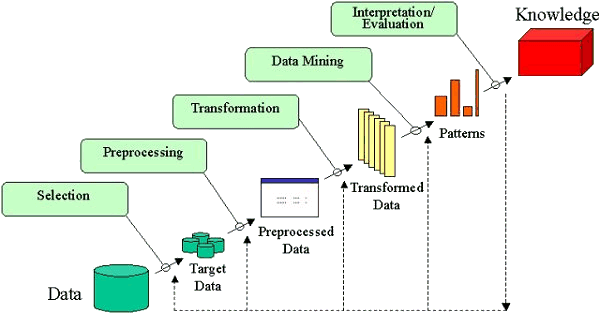
\includegraphics[width=0.82\textwidth]{figures/kdd_process.png}
\caption[Processus KDD]{Processus de méthodologie Knowledge Discovery in Databases (KDD)}
\label{fig:kdd_process}
\end{figure}

\subsection{SEMMA}

La méthode \textbf{SEMMA} (Sample, Explore, Modify, Model, Assess), développée
par SAS Institute, est largement utilisée dans les projets industriels de
science des données. Elle met l'accent sur la préparation, l'exploration et la
modélisation statistique des données. Elle comprend cinq étapes :
\begin{itemize}
  \item \textbf{Sample} : sélectionner un sous-ensemble représentatif des données ;
  \item \textbf{Explore} : analyser les tendances, anomalies et relations significatives ;
  \item \textbf{Modify} : transformer les données et créer des variables pertinentes ;
  \item \textbf{Model} : appliquer des algorithmes de modélisation ;
  \item \textbf{Assess} : tester et valider la performance des modèles.
\end{itemize}

\begin{figure}[H]
\centering
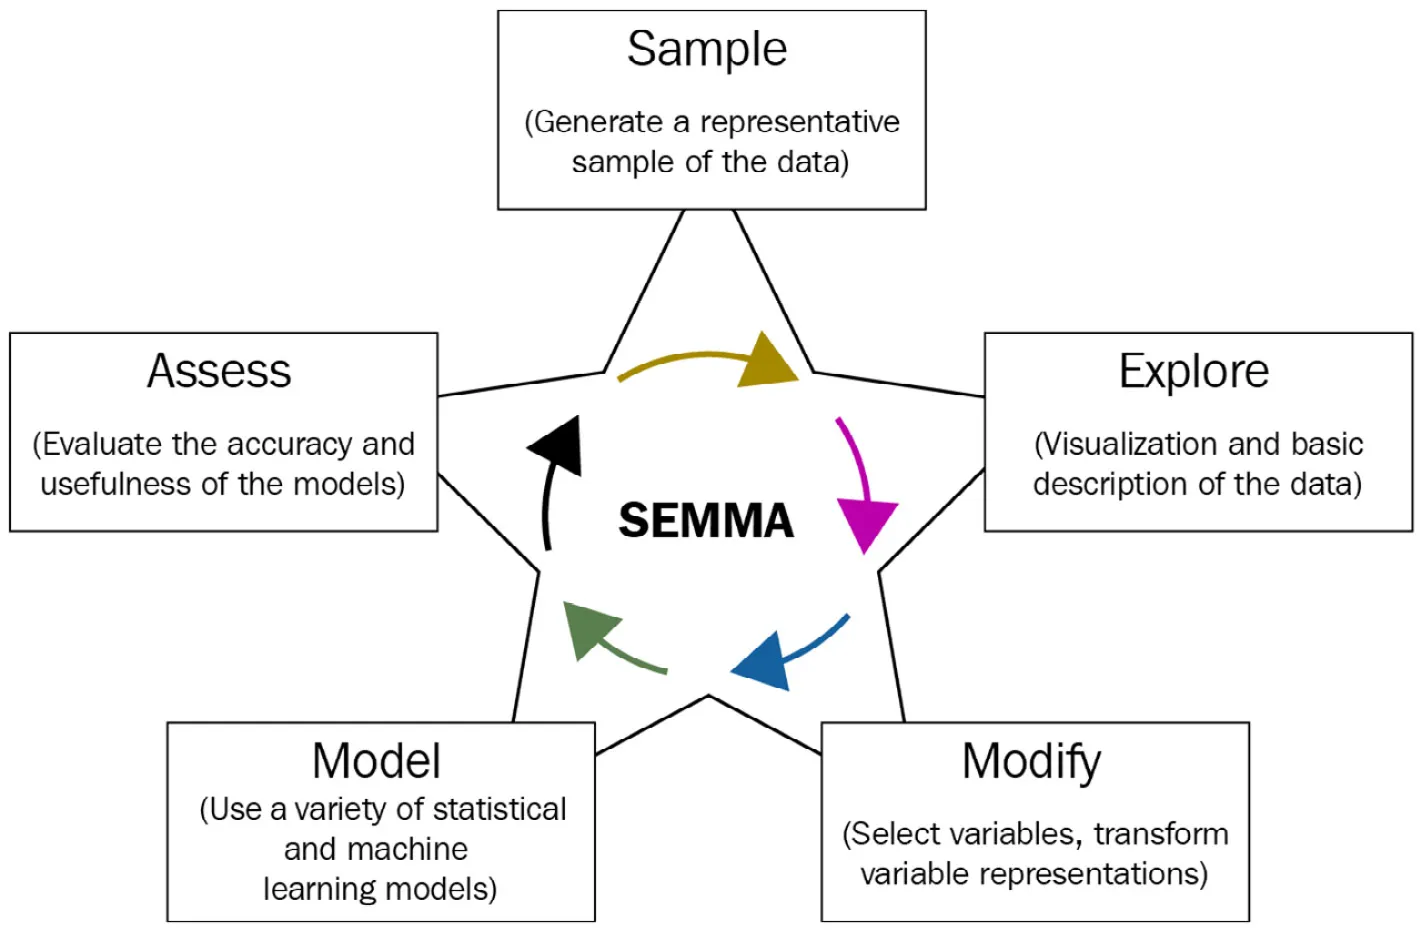
\includegraphics[width=0.82\textwidth]{figures/semma_process.png}
\caption[Processus SEMMA]{Processus d'exploration de données SEMMA}
\label{fig:semma_process}
\end{figure}

\subsection{CRISP-DM}

La méthodologie \textbf{CRISP-DM} (Cross-Industry Standard Process for Data
Mining) est un processus standardisé destiné à encadrer les projets de science
des données de manière structurée et reproductible. Elle repose sur une logique
cyclique et itérative permettant de revenir sur les phases précédentes lorsque
les résultats ou les contraintes métier l'exigent.

Le processus CRISP-DM comprend six étapes :
\begin{itemize}
  \item compréhension du métier ;
  \item compréhension des données ;
  \item préparation des données ;
  \item modélisation ;
  \item évaluation ;
  \item déploiement.
\end{itemize}

\begin{figure}[H]
\centering
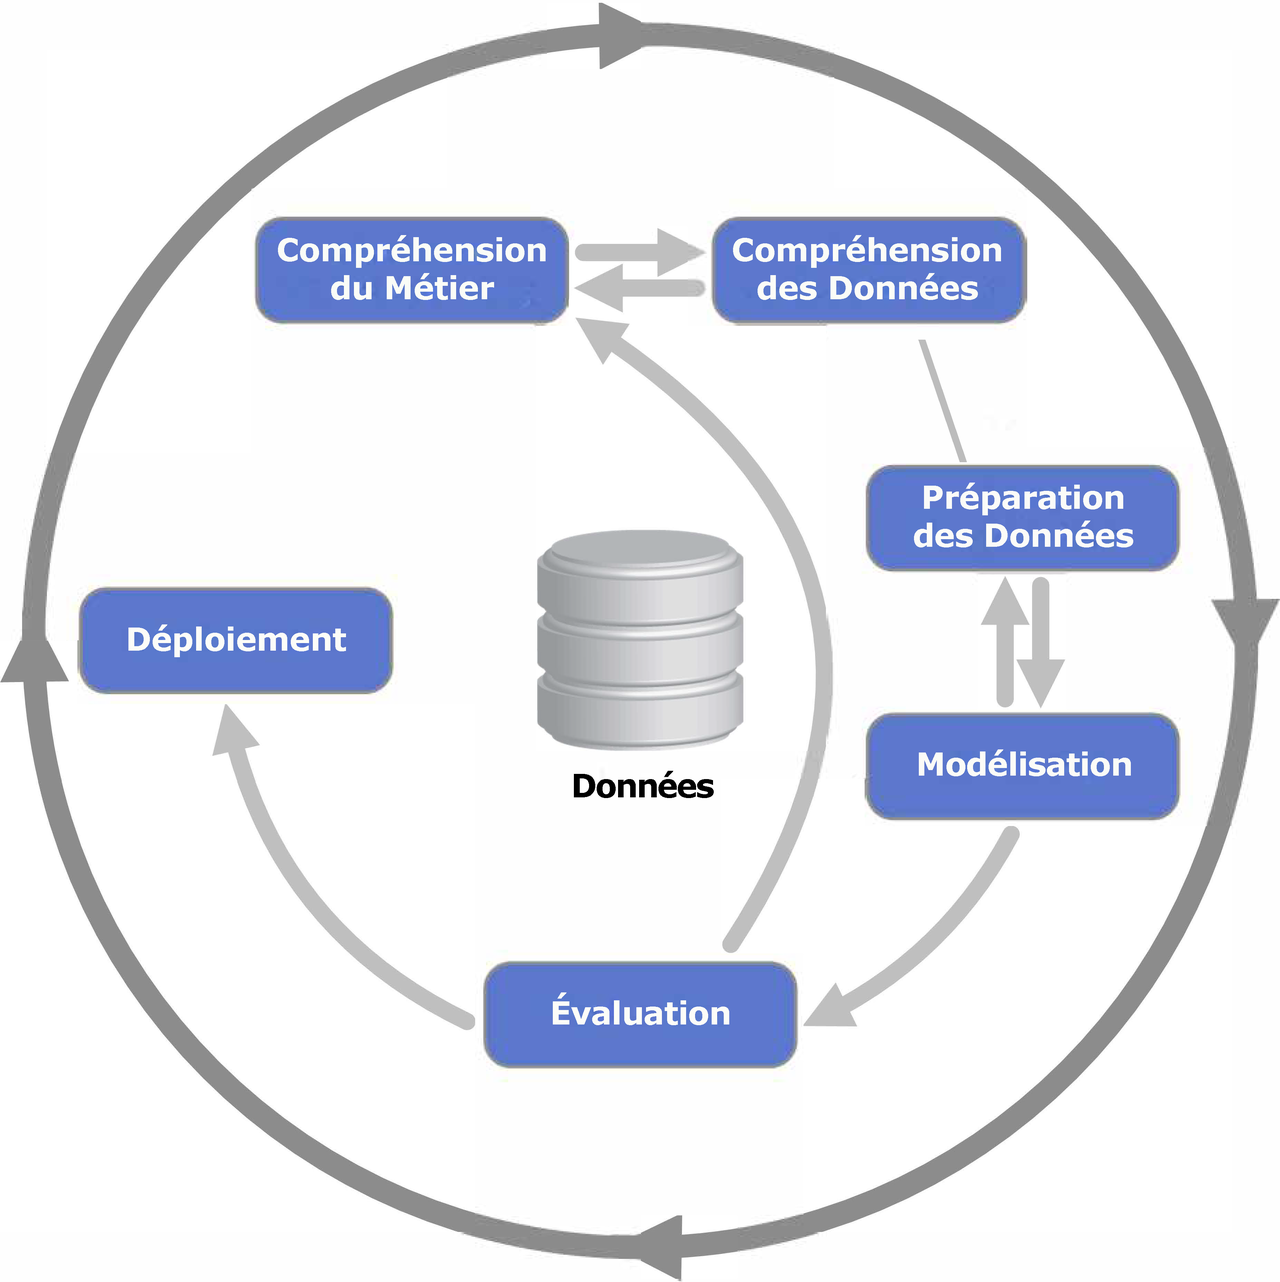
\includegraphics[width=0.72\textwidth]{figures/crispdm_process.png}
\caption[Processus CRISP-DM]{Processus de méthodologie Cross-Industry Standard Process for Data Mining (CRISP-DM)}
\label{fig:crispdm_process}
\end{figure}

\subsection{Choix de la méthodologie}

Après l'étude des méthodologies KDD, SEMMA et CRISP-DM, une comparaison est
nécessaire afin d'identifier l'approche la plus adaptée au projet Smart Farm AI.

\begin{table}[H]
\centering
\caption{Comparaison des méthodologies KDD, SEMMA et CRISP-DM}
\label{tab:comparaison_methodologies}
\renewcommand{\arraystretch}{1.2}
\resizebox{\textwidth}{!}{%
\begin{tabular}{p{0.18\textwidth}p{0.25\textwidth}p{0.25\textwidth}p{0.25\textwidth}}
\toprule
\textbf{Aspect} & \textbf{KDD} & \textbf{SEMMA} & \textbf{CRISP-DM} \\
\midrule
Étapes & Sélection, prétraitement, transformation, exploration, interprétation/évaluation & Échantillonner, explorer, modifier, modéliser, évaluer & Compréhension métier, compréhension des données, préparation, modélisation, évaluation, déploiement \\
Compréhension métier & Non incluse explicitement & Non incluse explicitement & Incluse dès la première phase \\
Déploiement & Peu détaillé & Non inclus explicitement & Inclus comme phase finale \\
Flexibilité & Séquence relativement fixe & Séquence relativement fixe & Transitions itératives entre phases \\
Orientation & Découverte de connaissances & Modélisation statistique et outil SAS & Guide complet orienté métier et produit \\
Résultat de l'étude & Approche fondatrice & Approche opérationnelle pour la modélisation & Approche la plus complète pour ce projet \\
\bottomrule
\end{tabular}%
}
\end{table}

\begin{table}[H]
\centering
\caption{Avantages et inconvénients des méthodologies étudiées}
\label{tab:avantages_inconvenients_methodologies}
\renewcommand{\arraystretch}{1.2}
\resizebox{\textwidth}{!}{%
\begin{tabular}{p{0.18\textwidth}p{0.38\textwidth}p{0.38\textwidth}}
\toprule
\textbf{Méthode} & \textbf{Avantages} & \textbf{Inconvénients} \\
\midrule
KDD & Processus interactif et itératif, adapté à la découverte de connaissances & Prend peu en compte les aspects métier et le déploiement opérationnel \\
SEMMA & Cadre clair pour explorer, modifier et modéliser les données & N'intègre pas explicitement l'utilisation métier des connaissances découvertes \\
CRISP-DM & Modèle hiérarchique, flexible, largement utilisé et orienté métier & Décrit les phases à suivre mais reste moins précis sur les outils et les boucles de rétroaction \\
\bottomrule
\end{tabular}%
}
\end{table}

Au regard de cette comparaison, CRISP-DM est retenue comme méthodologie
principale du projet. Elle est adaptée à Smart Farm AI car elle relie les
objectifs métier, la compréhension des données, la modélisation, l'évaluation et
le déploiement opérationnel. Elle est complétée par une organisation Scrum afin
de structurer le développement logiciel en sprints courts et itératifs.

\subsection{Adaptation CRISP-DM/Scrum au projet}

La méthodologie \textbf{CRISP-DM} a été adoptée pour la composante science des
données, tandis que \textbf{Scrum} a été utilisé pour organiser le développement
logiciel. Cette combinaison permet de concilier rigueur analytique et agilité de
réalisation.

\begin{description}
  \item[Compréhension métier] Identification des indicateurs critiques
  (FCR, taux de mortalité, production d'œufs) avec les utilisateurs cibles ;
  \item[Compréhension des données] Analyse des journaux IoT, historiques de production,
  images annotées et documents vétérinaires ;
  \item[Préparation des données] Nettoyage, normalisation, traitement des valeurs
  manquantes et constitution des jeux d'entraînement ;
  \item[Modélisation] Entraînement YOLOv11, modèles prédictifs avicoles et pipeline RAG+LLM ;
  \item[Évaluation] Validation croisée, intervalles de confiance, métriques BLEU/ROUGE
  et Cohen's Kappa ;
  \item[Déploiement] Conteneurisation Docker, monitoring WebSocket et mise à disposition
  via PWA.
\end{description}

\begin{figure}[H]
\centering
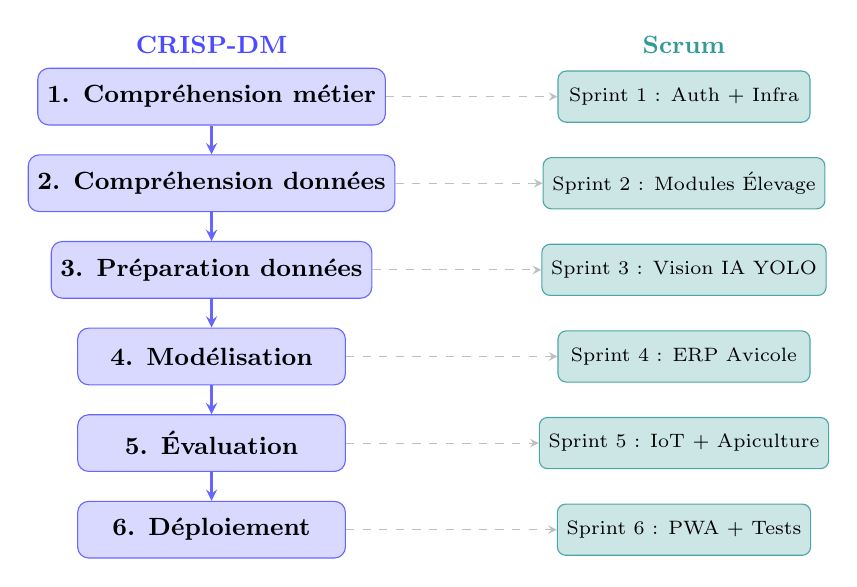
\begin{tikzpicture}[
  phase/.style={rectangle, rounded corners=4pt, minimum width=3.4cm,
                minimum height=0.72cm, text centered, align=center, font=\small\bfseries,
                draw=blue!60, fill=blue!15},
  sprint/.style={rectangle, rounded corners=3pt, minimum width=3.2cm,
                 minimum height=0.65cm, text centered, align=center, font=\scriptsize,
                 draw=teal!70, fill=teal!20},
  arr/.style={->, >=stealth, thick, blue!60},
  link/.style={->, >=stealth, gray!50, dashed},
]
\node[phase] (c1) at (0,0)    {1. Compréhension métier};
\node[phase] (c2) at (0,-1.1) {2. Compréhension données};
\node[phase] (c3) at (0,-2.2) {3. Préparation données};
\node[phase] (c4) at (0,-3.3) {4. Modélisation};
\node[phase] (c5) at (0,-4.4) {5. Évaluation};
\node[phase] (c6) at (0,-5.5) {6. Déploiement};
\draw[arr] (c1)--(c2); \draw[arr] (c2)--(c3); \draw[arr] (c3)--(c4); \draw[arr] (c4)--(c5); \draw[arr] (c5)--(c6);
\node[sprint] (s1) at (6,0)    {Sprint 1 : Auth + Infra};
\node[sprint] (s2) at (6,-1.1) {Sprint 2 : Modules Élevage};
\node[sprint] (s3) at (6,-2.2) {Sprint 3 : Vision IA YOLO};
\node[sprint] (s4) at (6,-3.3) {Sprint 4 : ERP Avicole};
\node[sprint] (s5) at (6,-4.4) {Sprint 5 : IoT + Apiculture};
\node[sprint] (s6) at (6,-5.5) {Sprint 6 : PWA + Tests};
\draw[link] (c1.east)--(s1.west); \draw[link] (c2.east)--(s2.west); \draw[link] (c3.east)--(s3.west);
\draw[link] (c4.east)--(s4.west); \draw[link] (c5.east)--(s5.west); \draw[link] (c6.east)--(s6.west);
\node[font=\small\bfseries, blue!70]  at (0, 0.65)  {CRISP-DM};
\node[font=\small\bfseries, teal!80]  at (6, 0.65)  {Scrum};
\end{tikzpicture}
\caption[Alignement CRISP-DM/Scrum]{Alignement CRISP-DM/Scrum du projet Smart Farm AI}
\label{fig:crisp_scrum}
\end{figure}

\subsection{Planification des sprints}

\begin{table}[H]
\centering
\caption{Carnet de produit Smart Farm AI (récits utilisateur prioritaires)}
\label{tab:product_backlog}
\resizebox{\textwidth}{!}{%
\begin{tabular}{cllcc}
\toprule
\textbf{Identifiant} & \textbf{Acteur} & \textbf{Récit utilisateur} & \textbf{Priorité} & \textbf{Points} \\
\midrule
US-01 & Éleveur  & Visualiser le tableau de bord de la ferme avec alertes en temps réel & Obligatoire & 8 \\
US-02 & Éleveur  & Analyser une image d'animal avec l'IA YOLO et recevoir un conseil en Darija & Obligatoire & 13 \\
US-03 & Éleveur  & Gérer les lots avicoles (FCR, mortalité, ponte, vente) & Obligatoire & 13 \\
US-04 & Éleveur  & Surveiller les ruches via la télémétrie IoT & Obligatoire & 8 \\
US-05 & Travailleur & Consulter les tâches assignées depuis l'application mobile hors connexion & Obligatoire & 5 \\
US-06 & Travailleur & S'authentifier par OTP WhatsApp sans mot de passe & Obligatoire & 5 \\
US-07 & Éleveur  & Localiser les vétérinaires et les marchés sur la carte SIG & Souhaitable & 5 \\
US-08 & Éleveur  & Recevoir des alertes d'urgence sur WhatsApp & Souhaitable & 8 \\
US-09 & Éleveur  & Exporter des rapports en PDF & Optionnel & 3 \\
US-10 & Éleveur  & Consulter les prévisions météo intégrées & Optionnel & 3 \\
\midrule
\multicolumn{4}{r}{\textbf{Total des points}} & \textbf{71} \\
\bottomrule
\end{tabular}%
}
\end{table}

\begin{table}[H]
\centering
\caption{Planification des sprints Smart Farm AI}
\label{tab:sprints}
\resizebox{\textwidth}{!}{%
\begin{tabular}{cllc}
\toprule
\textbf{Sprint} & \textbf{Période} & \textbf{Objectif principal} & \textbf{Points} \\
\midrule
S1 & Sem. 1--2  & Infrastructure : FastAPI, BDD PostgreSQL, authentification JWT/OTP & 13 \\
S2 & Sem. 3--4  & Gestion fermes, animaux, travailleurs ; RBAC & 13 \\
S3 & Sem. 5--6  & Module YOLO + agent Darija RAG/LLM & 13 \\
S4 & Sem. 7--8  & ERP avicole + modèles ML & 13 \\
S5 & Sem. 9--10 & IoT ESP32, MQTT, WebSocket ; apiculture & 13 \\
S6 & Sem. 11--12& PWA travailleur, SIG, tests, déploiement Docker+Caddy & 6 \\
\midrule
\multicolumn{3}{r}{\textbf{Total}} & \textbf{71} \\
\bottomrule
\end{tabular}%
}
\end{table}

\subsection{Planification -- Diagramme de Gantt}

\begin{figure}[H]
\centering
\resizebox{\textwidth}{!}{%
\begin{ganttchart}[
  x unit=0.78cm,
  y unit chart=0.65cm,
  vgrid,
  hgrid,
  title label font=\small\bfseries,
  bar label font=\small,
  group label font=\small\bfseries,
  milestone label font=\small\itshape,
  bar/.style={fill=blue!45, rounded corners=2pt},
  bar height=0.55,
  group/.style={fill=green!35, draw=green!70},
  milestone/.style={fill=red!65, rounded corners=2pt},
  title/.style={fill=blue!15, draw=none}
]{1}{12}
  \gantttitle{Smart Farm AI -- Planification 12 semaines}{12} \\
  \gantttitle{S1}{1}\gantttitle{S2}{1}\gantttitle{S3}{1}\gantttitle{S4}{1}%
  \gantttitle{S5}{1}\gantttitle{S6}{1}\gantttitle{S7}{1}\gantttitle{S8}{1}%
  \gantttitle{S9}{1}\gantttitle{S10}{1}\gantttitle{S11}{1}\gantttitle{S12}{1} \\
  \ganttgroup{Phase 1 -- Analyse \& Conception}{1}{3} \\
  \ganttbar{Étude de l'existant}{1}{1} \\
  \ganttbar{Analyse des besoins}{2}{2} \\
  \ganttbar{Architecture système}{3}{3} \\
  \ganttgroup{Phase 2 -- Développement}{4}{10} \\
  \ganttbar{Sprint~1 : Auth + Infra}{4}{4} \\
  \ganttbar{Sprint~2 : Fermes + Animaux}{5}{5} \\
  \ganttbar{Sprint~3 : YOLO + RAG}{6}{7} \\
  \ganttbar{Sprint~4 : ERP Avicole}{8}{8} \\
  \ganttbar{Sprint~5 : IoT + Apiculture}{9}{9} \\
  \ganttbar{Sprint~6 : PWA + Tests}{10}{10} \\
  \ganttgroup{Phase 3 -- Validation terrain}{11}{12} \\
  \ganttbar{Tests 7 fermes pilotes}{11}{11} \\
  \ganttbar{Analyse résultats + Rapport}{12}{12} \\
  \ganttmilestone{Rendu mémoire}{12}
\end{ganttchart}%
}
\caption[Diagramme de Gantt du projet]{Diagramme de Gantt du projet Smart Farm AI (12 semaines)}
\label{fig:gantt}
\end{figure}

\section*{Conclusion}
\phantomsection
\addcontentsline{toc}{section}{Conclusion}
Ce chapitre a posé les fondements conceptuels et méthodologiques du projet
Smart Farm AI. L'analyse de l'existant démontre l'originalité de la plateforme
face aux solutions commerciales internationales. La méthodologie hybride
CRISP-DM/Scrum garantit à la fois la rigueur scientifique de la composante
ML et l'agilité nécessaire au développement logiciel en milieu startup.

% ============================================================
%  CHAPITRE 2 : ANALYSE DES BESOINS ET ARCHITECTURE
% ============================================================
